\documentclass[12pt, a4paper]{article}   	
\usepackage{geometry}
\usepackage{amssymb}
\usepackage{mathtools}
\usepackage{amsmath}
\usepackage{amsthm}
\usepackage[utf8]{inputenc}
\usepackage{color}   
\usepackage{tikz}
\usepackage{tcolorbox}
\usepackage{multicol}
\usepackage[thinc]{esdiff}
\usepackage{physics}
\usepackage{bm}
\usepackage{pdfpages}
\usepackage{pdflscape}
\usepackage{listings}
\usepackage{float}

\usepackage{hyperref}

\hypersetup{colorlinks=true, linktoc=all, linkcolor=black,}

\usetikzlibrary{arrows.meta}

\newtheorem*{remark}{Remark}
\newtheorem*{note}{Note}

\theoremstyle{definition}
\newtheorem{definition}{Definition}[section]
\newtheorem{theorem}{Theorem}[section]
\newtheorem*{example}{Example}
\newtheorem{proposition}{Proposition}

\theoremstyle{plain}
\newtheorem{corollary}{Corollary}[theorem]
\newtheorem{lemma}[theorem]{Lemma}

\newcommand{\bb}[1]{\mathbb{#1}}
\newcommand{\f}[2]{\frac{#1}{#2}}
\newcommand{\imply}{\Rightarrow}
\newcommand{\conj}[1]{\overline{#1}}
\newcommand{\vect}[1]{\mathbf{#1}}
\newcommand{\Cal}[1]{\mathcal{#1}}

\DeclareMathOperator{\Span}{span}
\DeclareMathOperator{\im}{Im}
\DeclareMathOperator{\Ker}{Ker}

\title{LAG 1 Revision Notes}
\date{}
\author{Francesco Chotuck}
\begin{document} 
\maketitle 

\tableofcontents

\pagebreak

\section{Foundational material}

\subsection{Sums}

\subsubsection{Relabelling indices}

You can shift indices provided you also shift the bounds to match.

$$\sum_{k=1}^{n} (k-1) = \sum_{k=0}^{n-1} k$$

\subsubsection{Double Sums}

$$\left(\sum_{k=0}^{n} a_k \right)\left(\sum_{k=0}^{m} b_k \right) = \sum_{j=0}^{n} \sum_{k=0}^{m} a_jb_k$$

\subsubsection{Standard Sums}

\begin{itemize}

	\item $$\sum_{n=1}^{n} 1 = \underbrace{1+1+\ldots+1}_\text{n times} =n$$

	\item $$\sum_{n=1}^{n} k = 1+2+3+\ldots+n = \frac{1}{2}n(n+1)$$

	\item $$\sum_{n=1}^{n} r^k = \frac{r-r^{n+1}}{1-r} $$

\end{itemize}

\subsection{Complex Numbers}

\subsubsection{The Fundamental Theorem of Algebra}

Let $P$ be a polynomial of degree $n,$ i.e. $$P(z) = a_n z^n + a_{n-1} z^{n-1} + \ldots +a_1 z+ a_0,$$ where $a_0,\ldots,a_n \in \bb{C}.$ Then the equation $P(z) = 0$ has $n$ solutions $w_1,w_2,\ldots,w_n$ (some of the solutions may be repeated). This means that $P(z)$ can be factorised as $$P(z) = a_n(z-w_1)(z-w_2)\ldots(z-w_n).$$

\begin{remark}
A field that satisfies this property is called \textbf{algebraically closed}. Thus, $\bb{C}$ is algebraically closed whereas $\bb{R}$ is not.
\end{remark}

\subsubsection{Complex conjugate and modulus}

\textbf{Properties of complex conjugation:}
Let $z=a+ib$ and $w=c+id,$ where $a,b,c,d \in \bb{R}.$

\begin{enumerate}
	
	\item $\conj{z+w} = \conj{z}+\conj{w}.$

	\item $\conj{zw} = \conj{z} \, \conj{w}.$

	\item Re($z)= \frac{1}{2}(z+\conj{z}).$

	\item Im($z)= \frac{1}{2i}(z-\conj{z}).$ 

\end{enumerate}

\textbf{Properties of the modulus:}

\begin{enumerate}
	
	\item $|z| = \sqrt{z\conj{z}}.$

	\item $|z|$ is always a non-negative real number.

	\item $|z|=|\conj{z}|.$

	\item $|\text{Re}(z)|\leq|z|$ and $|\text{Im}(z)|\leq|z|$ since $a^2\leq a^2+b^2$ and $b^2\leq a^2+b^2.$

	\item $|zw| = |z||w|.$

\end{enumerate}

\begin{proposition}(The triangle inequality). For every $z,w \in \bb{C},$ $$|z+w|\leq|z|+|w|.$$ \end{proposition}

\subsubsection{Euler's Formula}

\begin{theorem}(Euler's Formula) For every $\theta \in \bb{R},$ $$e^{i\theta} = \cos{\theta}+i\sin{\theta}.$$ \end{theorem}

Therefore, a complex number $z=re^{i\theta}$ where $r=|z|$ and arg($z)=\theta.$

\begin{remark}
The argument of $z$ i.e. $\theta$ lies in the interval $-\pi<\theta\leq \pi.$
\end{remark}

\subsubsection{De Moivre's theorem}

\begin{theorem}(De Moivre's theorem). For every $\theta \in \bb{R}$ and $n \in \bb{N},$ $$(\cos{\theta}+i\sin{\theta})^n=\cos(n\theta)+i\sin(n\theta).$$ \end{theorem}

\subsubsection{Roots of Unity}

\begin{proposition} Let $n$ be a positive integer. The equation $z^n=1$ has exactly $n$ distinct roots in the complex numbers and they are $$z=e^{\frac{i2\pi k}{n}}, \quad k=0,1,2,\ldots,n-1.$$ \end{proposition}

\begin{remark}
Sketching the roots of unity on an Argand diagram form a $n$-polygon.
\end{remark}
	
\begin{proposition} Let $n$ be an integer with $n\geq2.$ The sum of the $n$-th roots of unity is equal to zero, i.e. $$\sum_{k=0}^{n-1} e^{\frac{i2\pi k}{n}}=0.$$ \end{proposition}

\subsubsection{Logarithms and complex powers}

\begin{definition} Let $z \in \bb{C}, z \neq 0.$ Then the \textbf{principal logarithm} of $z$ is denoted Log $z$ and defined by $$\text{Log }z = \log{|z|}+i\text{Arg }z.$$ \end{definition}
 
\section{Vectors}

A vector is an object contained in a vector space, usually denoted as a column or a row of entries/components in $\bb{R}$ or $\bb{C}.$

\subsection{Linear combinations and span}

\begin{definition} Let $\vect{v}_1,\vect{v}_2,\ldots,\vect{v}_m$ be vectors in $\bb{R}^n.$ A \textbf{linear combination} of $\vect{v}_1,\vect{v}_2,\ldots,\vect{v}_m$ is an expression of the form $$\alpha_1\vect{v}_1+\alpha_2\vect{v}_2+\ldots+\alpha_m\vect{v}_m=\sum_{k=1}^{m} \alpha_m\vect{v}_m,$$ where $\alpha_1,\ldots,\alpha_n$ are scalars (in $\bb{R}^n$). \end{definition}

\begin{definition} Let $\vect{v}_1,\vect{v}_2,\ldots,\vect{v}_m$ be vectors in $\bb{R}^n.$ The \textbf{linear span} of $\vect{v}_1,\vect{v}_2,\ldots,\vect{v}_m$ is the set of all vectors which are linear combinations of $\vect{v}_1,\vect{v}_2,\ldots,\vect{v}_m.$ We denote the linear span of $\vect{v}_1,\vect{v}_2,\ldots,\vect{v}_m$ by $\Span\{\vect{v}_1,\vect{v}_2,\ldots,\vect{v}_m\},$ i.e. $$\Span\{\vect{v}_1,\vect{v}_2,\ldots,\vect{v}_m\} = \left\{\sum_{k=1}^{m} \alpha_k\vect{v}_k : \alpha_1,\ldots,\alpha_m \in \bb{R}\right\}$$ \end{definition} 

Some examples:

\begin{itemize}

	\item Let $\vect{v} \in \bb{R}^n$ be a non-zero vector. Then $$\Span\{\vect{v}\}=\{\alpha\vect{v}:\alpha \in \bb{R}^n\}.$$ Geometrically, this is a line. In fact it is the line through the origin in the direction of the vector $\vect{v}.$ Moreover, every line through the origin is of this form.

	\item Let $\vect{v}, \vect{w} \in \bb{R}^n$ be a non-zero vectors. Then $$\Span\{\vect{v},\vect{w}\}=\{\alpha\vect{v}+\beta\vect{w}:\alpha,\beta \in \bb{R}^n\}.$$ Geometrically, this is a plane containing $\vect{v},\vect{w}$ and the origin. However, if $\vect{w}$ is a multiple of $\vect{v},$ then $\Span\{\vect{v},\vect{w}\}= \Span\{\vect{v}\}$ and so we a get a line again and vice versa.

\end{itemize}

\subsection{Lengths and Dot Product}

\begin{definition} Let $\vect{v}=(v_1,v_2,\ldots,v_n) \in \bb{R}^n.$ The \textbf{length} or \textbf{norm} of $\vect{v}$ is denoted $||\vect{v}||$ and defined by $$\sqrt{\sum_{k=1}^{n} v_k^2} = \sqrt{v_1^2+v_2^2+\ldots+v_n^2}. $$ \end{definition}

We can define the distance between two points $\vect{u}$ and $\vect{v}$ in $\bb{R}^n$ to be $||\vect{v-u}||.$

\begin{proposition} (Properties of the norm). For every $\vect{u},\vect{v} \in \bb{R}^n$ and every scalar $\alpha$ we have 

\begin{itemize}

	\item $||\vect{v}||\geq0$ and $||\vect{v}||=0$ if and only if $\vect{v}=\vect{0},$

	\item $||\alpha\vect{v}||=|\alpha|\,||\vect{v}||,$

	\item $||\vect{u+v}||\leq||\vect{u}||+||\vect{v}||.$

\end{itemize}

\end{proposition}

\begin{definition} Let $\vect{u}=(u_1,\ldots,u_n), \vect{v}=(v_1,\ldots,v_n) \in \bb{R}^n.$ Then the \textbf{dot product} (or \textbf{scalar product} or \textbf{inner product}) of $\vect{u}$ and $\vect{v}$ is denoted $\vect{u}\cdot \vect{v}$ and defined by $$\vect{u}\cdot\vect{v} = \sum_{k=1}^{n}u_kv_k =v_1u_1+u_2v_2+\ldots+u_nv_n.$$ \end{definition}

\begin{proposition} (Properties of the dot product). For every $\vect{u},\vect{v},\vect{w} \in \bb{R}^n$ and every scalar $\alpha$ we have 

\begin{itemize}

	\item $||\vect{v}||= \sqrt{\vect{v}\cdot \vect{v}},$

	\item $\vect{v}\cdot\vect{v} \geq0$ and $\vect{v}\cdot\vect{v}=0 \iff \vect{v}=0,$

	\item $\vect{u}\cdot\vect{v}=\vect{v}\cdot\vect{u},$

	\item $\vect{u}\cdot(\vect{v+w}) = \vect{u\cdot v}+ \vect{u\cdot w },$

	\item $(\alpha\vect{u})\cdot \vect{v}=\alpha(\vect{u \cdot v}) = \vect{u} \cdot (\alpha \vect{v}).$

\end{itemize}

\end{proposition}

\begin{proposition} Let $\vect{u},\vect{v} \in \bb{R}^n$ with $n=2,3$ and let $\theta$ be the angle between $\vect{u}$ and $\vect{v}.$ Then $$\vect{u\cdot v} = ||\vect{u}|| \, ||\vect{v}||\cos{\theta}.$$ \end{proposition}

\begin{remark} \hphantom{This is to make the text look nice.}
\begin{enumerate}
	
	\item In particular, we have that two non-zero vectors $\vect{u}$ and $\vect{v}$ are perpendicular (or \textit{orthogonal} for $\bb{R}^3$) if and only if $\vect{u\cdot v}=0.$

	\item Since $|\cos{\theta}|\leq 1,$ we have that $$|\vect{u\cdot v}|\leq ||\vect{u}|| \, ||\vect{v}||.$$ This is known as the \textit{Cauchy-Schwartz} inequality (check LAG 2).

\end{enumerate}
\end{remark} 


\subsubsection{Length and dot product with complex numbers}

\begin{definition} Let $\vect{z}=(z_1,z_2,\ldots,z_n) \in \bb{C}^n.$ The \textbf{length} or \textbf{norm} of $\vect{z}$ is denoted $||\vect{z}||$ and defined by $$\sqrt{\sum_{k=1}^{n} ||z_k||^2} = \sqrt{|z_1|^2+|z_2|^2+\ldots+|z_n|^2}.$$ \end{definition}

We can define the distance between two point $\vect{z}$ and $\vect{w}$ in $\bb{C}^n$ to be $||\vect{z-w}||.$

\begin{definition} Let $\vect{z}=(z_1,\ldots,z_n), \vect{w}=(w_1,\ldots,w_n) \in \bb{C}^n.$ Then the \textbf{dot product} (or \textbf{scalar product} or \textbf{inner product}) of $\vect{z}$ and $\vect{w}$ is denoted $\vect{z}\cdot \vect{w}$ and defined by $$\vect{z}\cdot\vect{w} = \sum_{k=1}^{n}z_k\conj{w_k} =z_1\conj{w_1}+z_2\conj{w_2}+\ldots+z_n\conj{w_n}.$$ \end{definition}

\begin{remark}
If the entries of $\vect{z}$ and $\vect{w}$ are real, the definition of the dot product in $\bb{C}^n$ and $\bb{R}^n$ coincide. This is because in this case $\conj{w_k}=w_k$ and so $$\sum_{k=1}^{n} z_k\conj{w_k} = \sum_{k=1}^{n}z_k w_k.$$
\end{remark}
 
\subsection{Lines and Planes}

Let $L$ be a line through the point $\vect{v}_0$ and parallel to $\vect{p}.$ Then every point $\vect{v}$ on $L$ is of the form $$\vect{v}=\vect{v}_0+t\vect{p}$$ for some $t \in \bb{R}.$ As the real parameter $t$ varies, we get every point on the line. 

\begin{center}
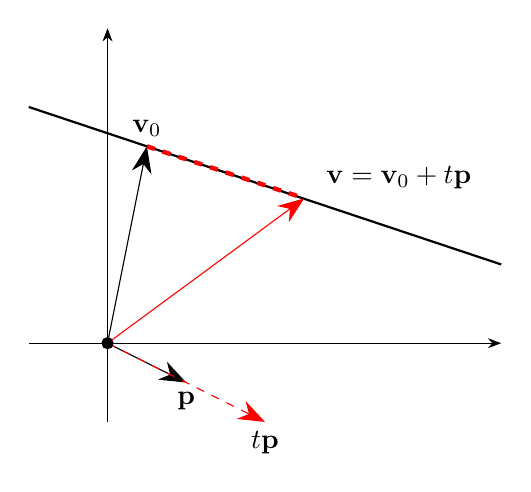
\begin{tikzpicture}
%\draw [help lines] (-4,-4) grid (5,4);
\draw [-Stealth] (-1,-2) -- (-1,3);
\draw [-Stealth] (-2,-1) -- (4,-1);
\draw [thick] (-2,2) -- (4,0);
\draw [-{Stealth[scale=2]}] (-1,-1) -- (0,-1.5);
\draw [-{Stealth[scale=2]}][dashed][red] (-1,-1) -- (1,-2);
\draw [-{Stealth[scale=2]}] (-1,-1) -- (-0.5,1.5);
\draw [-{Stealth[scale=2]}][red] (-1,-1) -- (1.5,0.84);
\draw [dashed][red][ultra thick] (-0.5,1.5) -- (1.5,0.84);
\node [below] at (0,-1.5) {$\vect{p}$};
\node [below] at (1,-2) {$t\vect{p}$};
\node [above] at (-0.5,1.5) {$\vect{v}_0$};
\node [above] at (2.7,0.84) {$\vect{v}=\vect{v}_0+t\vect{p}$};
%\filldraw [black] (0,0) circle (2pt);
\filldraw [black] (-1,-1) circle (2pt);
\end{tikzpicture}
\end{center}

Any point $\vect{v}$ on the line can be expressed in the form $\vect{v}=\vect{v}_0+t\vect{p}$ for some choice of $t \in \bb{R}.$

A plane can also be expressed parametrically as $$\vect{v}=\vect{v}_0+t\vect{p}+s\vect{q}$$ for some $t,s \in \bb{R},$ if and only if $\vect{p}$ is not a multiple of $\vect{q}.$

\begin{remark}
The equation of a line and plane is not unique.
\end{remark}

\begin{proposition} A plane in $\bb{R}^3$ is the set of points $\vect{v}=(v_1,v_2,v_3)$ satisfying an equation $$av_1+bv_2+cv_3=d,$$ where $a,b,c,d \in \bb{R}$ are constants and $a,b,c$ not all zero.\end{proposition}

\begin{note}
The Cartesian equation of a plane is obtained by evaluating the dot product the vector equation of a plane $\vect{v}=\vect{v}_0+t\vect{p}+s\vect{q}$ by a vector $\vect{u}$ which is perpendicular to the plane. This is because $\vect{u \cdot p}=\vect{u \cdot q} = 0$ therefore, $\vect{u \cdot v}= \vect{u \cdot v_0}.$ Setting $d=\vect{u \cdot v_0}$ we obtain $av_1+bv_2+cv_3=d$ since, $\vect{u}=(a,b,c).$
\end{note}

\section{Vector Spaces}

\begin{definition} A \textbf{vector space} is any collection of objects $V$ (called \textbf{vectors}) for which two operations can be performed:

\begin{itemize}

	\item \textbf{Vector addition}, which takes two vectors $\vect{v,w} \in V$ and returns another vector $\vect{v+w} \in V$ (V is \textbf{closed under addition}).

	\item \textbf{Scalar multiplication}, which takes a vector $\vect{v} \in V$ and a scaler $\alpha \in \bb{F}$ and returns a vector $\alpha\vect{v} \in V$ (V is \textbf{closed under scalar multiplication}).

\end{itemize}

Furthermore, the following properties (or \textbf{axioms}) must be satisfied.

\begin{enumerate}
	
	\item Commutativity: $\vect{v+w=w+v}$ for all $\vect{v,w} \in V$;

	\item Associativity: $(\vect{u+v})+\vect{w}=\vect{u}+(\vect{v+w})$ for all $\vect{u,v,w};$

	\item Zero vector: there exists a vector, denoted $\vect{0}$ such that $\vect{v+0=v}$ for all $\vect{v} \in V$;

	\item Additive inverse: For every vector $\vect{v} \in V,$ there is a vector $\vect{-v} \in V$ such that $\vect{-v+v=0}$;

	\item Multiplicative identity: $1\vect{v=v}$ for all $\vect{v} \in V$;

	\item Multiplicative associativity: $\alpha(\beta\vect{v})=(\alpha\beta)\vect{v}$ for all $\vect{v} \in V$ and all $\alpha,\beta \in \bb{F};$

	\item Distributivity: $\alpha(\vect{v+w})=\alpha\vect{v}+\alpha\vect{w}$ for all $\vect{v,w} \in V$ and all $\alpha \in \bb{F};$ \\
	$(\alpha+\beta)\vect{v}=\alpha\vect{v}+\beta\vect{v}$ for all $\vect{v}\in V$ and all $\alpha,\beta \in \bb{F}.$

\end{enumerate}

\end{definition}

\subsection*{Examples of vector spaces}

\begin{itemize}
	
	\item Column Vectors;

	\item Zero vector space;

	\item Polynomials (usually denoted $\bb{P}_n$);

	\item Functions 

	\item Solutions to differential equations (this applies only to linear homogenous ODEs.

\end{itemize}

\subsection{Subspace}

\begin{definition} Let $V$ be a vector space. A non-empty set $W \subseteq V$ is a \textbf{subspace} of $V$ if 

\begin{enumerate}
	
	\item for every $\vect{u,v}\in W, \vect{u+v} \in W$ (W is closed under addition);

	\item for every $\alpha \in \bb{F}$ and $\vect{v} \in W, \alpha\vect{v} \in W$ (W is closed under scalar multiplication).

\end{enumerate}

\end{definition}

\begin{remark}
$W$ is a subspace of $V$ if $W$ is a vector space and a subset of $V.$
\end{remark} 

\begin{proposition} Let $\vect{v}_1,\vect{v}_2,\ldots,\vect{v}_n$ be vectors in $V.$ Then $\Span\{\vect{v}_1,\vect{v}_2,\ldots,\vect{v}_n\}$ is a subspace of $V.$ Moreover, if $W$ is any subspace of $V$ containing $\vect{v}_1,\vect{v}_2,\ldots,\vect{v}_n,$ then $W$ must contain $\Span\{\vect{v}_1,\vect{v}_2,\ldots,\vect{v}_n\}$ \end{proposition}

\subsection{Bases} 

\begin{definition} A collection of vectors $\vect{v}_1,\vect{v}_2,\ldots,\vect{v}_n \in V$ is a \textbf{basis} for $V$ if every vector $\vect{v}\in V$ admits a \textbf{unique} representation as a linear combination $$\vect{v} = \alpha_1\vect{v}_1+\alpha_2\vect{v}_2+\ldots+\alpha_n\vect{v}_n = \sum_{k=1}^{n} \alpha_k\vect{v}_k.$$ The coefficients $\alpha_1,\alpha_2,\ldots,\alpha_n$ are called \textbf{coordinates} of $\vect{v}$ with respect to the basis $\vect{v}_1,\vect{v}_2,\ldots,\vect{v}_n.$ \end{definition}

\subsection*{Example of bases}

\begin{itemize}

	\item Let $V=\bb{F}^n$ the vectors $\vect{e}_1=(1,0,0,\ldots,0),\vect{e}_2=(0,1,0,\ldots,0), \ldots, \vect{e}_n=(0,0,0,\ldots,1)$ form a basis for $\bb{F}^n.$

	\item Let $V=\bb{P}_n$ the vectors $\vect{e}_0=1,\vect{e}_1=t,\vect{e}_2=t^2,\ldots,\vect{e}_n=t^n$ form a basis for $\bb{F}^n.$

\end{itemize}

\subsection{Coordinate vector}

\begin{definition} Let $V$ be a vector space with basis $\Cal{E}=\{\vect{e}_1,\vect{e}_2,\ldots,\vect{e}_n\}$ and let $\vect{v}=\alpha_1\vect{e}_1+\alpha_2\vect{e}_2+\ldots+\alpha_n\vect{e}_n \in V.$ Then the \textbf{coordinate vector} of $\vect{v}$ with respect to $\Cal{E}$ is the column vector $$[\vect{v}]_{\Cal{E}}:=\begin{pmatrix} \alpha_1 \\ \alpha_2 \\ \vdots \\ \alpha_n\end{pmatrix} \in \bb{F}^n.$$ \end{definition}

Thus we have a one-to-one correspondence (isomorphism) between $V$ and $\bb{F}^n:$ $$\vect{v} \longleftrightarrow [\vect{v}]_{\Cal{E}}.$$

\begin{remark}
Addition and Scalar multiplication; $$[\vect{v+w}]_{\Cal{E}}=[\vect{v}]_{\Cal{E}}+[\vect{v}]_{\Cal{E}} \quad \text{and} \quad [\beta\vect{v}]_{\Cal{E}}=\beta[\vect{v}]_{\Cal{E}}.$$
\end{remark}

\subsection{Spanning and linearly independent sets}

\begin{definition} We say that a collection of vectors $\vect{v}_1,\vect{v}_2,\ldots,\vect{v}_n \in V$ \textbf{spans} $V,$ or that is a \textbf{spanning} set (or \textbf{generating} set), if every vector $\vect{v} \in V$ admits a representation as a linear combination $$\vect{v} = \alpha_1\vect{v}_1+\alpha_2\vect{v}_2+\ldots+\alpha_n\vect{v}_n = \sum_{k=1}^{n} \alpha_k\vect{v}_k.$$ Equivalently, $\vect{v}_1,\vect{v}_2,\ldots,\vect{v}_n \Span{V}$ if $$\Span\{\vect{v}_1,\vect{v}_2,\ldots,\vect{v}_n\}=V.$$
\end{definition}

\begin{remark}
One can always add additional vectors to a spanning set and still get a spanning set. However, removing a vector from a spanning set may cause it to stop spanning.
\end{remark} 

\begin{definition} A collection of vectors $\vect{v}_1,\vect{v}_2,\ldots,\vect{v}_n \in V$ are \textbf{linearly dependent} if there exists $\alpha_1,\alpha_2,\ldots,\alpha_n \in \bb{F}^n,$ not all zero, such that $$\alpha_1\vect{v}_1+\alpha_2\vect{v}_2+\ldots+\alpha_n\vect{v}_n =0.$$ The vectors $\vect{v}_1,\vect{v}_2,\ldots,\vect{v}_n \in V$ are \textbf{linearly independent} if they are not linearly dependent. \end{definition}

\begin{remark}
A collection of vectors is said to be linearly independent if there is precisely one representation of $\vect{0}$ as a linear combination i.e. it is unique implying $\alpha_1=\alpha_2=\ldots=\alpha_n=0.$
\end{remark}

\begin{proposition} The vectors $\vect{v}_1,\vect{v}_2,\ldots,\vect{v}_n \in V$ are linearly dependent if and only if one of the vectors can be represented as a linear combination of the others. \end{proposition}

\begin{remark}
Suppose $\vect{v}_1,\vect{v}_2,\ldots,\vect{v}_n$ are linearly dependent, then by Proposition 3.2 one of the vectors, say $\vect{v}_1,$ is a linear combination of the others. Then any of the vectors can be written as a linear combination of $\vect{v}_1,\vect{v}_2,\ldots,\vect{v}_n$ can also be written as a linear combination of $\vect{v}_2,\vect{v}_3,\ldots,\vect{v}_n$ i.e. $$\Span\{\vect{v}_1,\vect{v}_2,\ldots,\vect{v}_n\}=\Span\{\vect{v}_2,\vect{v}_3,\ldots,\vect{v}_n\}.$$ Therefore, if $\vect{v}_1,\vect{v}_2,\ldots,\vect{v}_n$ are linearly dependent, then one of the $\vect{v}_k$ is a linear combination of the others and we can remove this vector without changing their linear span.
\end{remark} 

\begin{proposition} A collection of vectors $\vect{v}_1,\vect{v}_2,\ldots,\vect{v}_n \in V$ is a basis if and only if it is linearly independent and spans V. \end{proposition}

\begin{proposition} Any finite spanning set contains a basis. \end{proposition}

\subsection{Dimension}

\begin{definition} The dimension of a vector space $V$ is denoted $\dim{V}$ and defined to be the number of elements in a basis for $V.$ If $V$ consists of only the zero vector we set $\dim{V}=0$ and if $V$ does not have a finite basis we set $\dim{V}=\infty.$ \end{definition}

\begin{theorem}(Dimension theorem). Let $V$ be a vector space. Then every basis of $V$ has the same number of elements. Moreover, if $V$ has a basis of $n$ elements then 
\begin{itemize}

	\item any set of vectors in $V$ with less than $n$ elements doesn't span $V$;

	\item any set of vectors in $V$ with more than $n$ elements is linearly dependent.
\end{itemize}
\end{theorem}

\begin{proposition} Let $\vect{v}_1,\vect{v}_2,\ldots,\vect{v}_m \in V$ be linearly independent vectors in a finite dimensional vector space $V.$ If $\vect{v}_1,\vect{v}_2,\ldots,\vect{v}_m$ do not span $V,$ there exist vectors $\vect{v}_{m+1},\vect{v}_{m+2},\ldots,\vect{v}_n$ such that $\vect{v}_1,\vect{v}_2,\ldots,\vect{v}_n$ is a basis of $V.$ \end{proposition}

\begin{proposition} A collection of $n$ vectors in an $n$ dimensional vector space is spanning if and only if it is linearly independent.\end{proposition}

\begin{remark}
If we want to check if a collection of $n$ vectors in $\bb{F}^n$ is a basis, we only need to check that it is linearly independent (or that it is spanning).
\end{remark}

\section{Linear Maps}

\begin{definition} Let $V$ and $W$ be vector spaces over $\bb{F}$ (either both real or both complex). Then a map (or transformation) $T : V \rightarrow W$ is linear if it satisfies the following two conditions:
\begin{itemize}
	
	\item for every $\vect{u},\vect{v} \in V, T(\vect{u+v})=T(\vect{u})+T(\vect{v})$;

	\item for every $\vect{v} \in V$ and every $\alpha \in \bb{F},T(\alpha\vect{v})=\alpha T(\vect{v}).$

\end{itemize}
\end{definition}

\begin{remark}
Observe that we have two different addition rules in the above definition: $$T(\underbrace{\vect{u+v}}_\text{$+$ in $V$})=\underbrace{T(\vect{u})+T(\vect{v})}_\text{$+$ in $W$}$$
\end{remark}

\subsection*{Examples of linear maps}

\begin{itemize}

	\item Identity map;

	\item Zero map

	\item Reflection

	\item Rotation 

	\item Differentiation

\end{itemize}

\subsection{Operations on linear maps}

\subsubsection*{Addition}

Let $V$ and $W$ be vectors spaces (over $\bb{F}$) and let $S:V \rightarrow W$ and $T :V \rightarrow W$ be linear maps (note that they have the same domain and range). We can add $S$ and $T$ by the rule $$(S+T)(\vect{v})=S(\vect{v})+T(\vect{v}) \quad \text{for all} \quad \vect{v} \in V.$$

\begin{remark}
The map $(S+V)$ is a linear map.
\end{remark}

\subsubsection*{Scalar multiplication}

Multiplying a linear map $T :V \rightarrow W$ by a scalar $\alpha \in \bb{F}$ according to the rule $$(\alpha T)(\vect{v})=\alpha T(\vect{v}).$$

\begin{remark}
The map $\alpha T$ is a linear map.
\end{remark} 

\subsubsection*{Composition}

Let $U,V$ and $W$ be vector spaces and let $S : U \rightarrow V$ and $T : V \rightarrow W$ be linear maps (note that the range of $S$ is the domain of $T$). We can consider the map we obtain by first applying $S$ and then applying $T,$ i.e. the map $T \circ S : U \rightarrow W$ defined by $$(T\circ S)(\vect{u})=T(S(\vect{u})) \quad \text{for all} \quad \vect{u} \in U$$

\begin{remark}
The map $T\circ S$ is a linear map.
\end{remark}

\section{Matrices}

\subsection{Matrix of a linear map between general vector spaces}

Let $V$ and $W$ be vector spaces with $\dim{V} = n$ and $\dim{W} = m.$ Suppose that we fix bases $\Cal{E} = \{\vect{e}_1,\vect{e}_2,...,\vect{e}_n\}$ and $\Cal{F} = \{\vect{f}_1,\vect{f}_2,...,\vect{f}_m\}$ of $V$ and $W$ respectively. Then we can get a matrix for a linear map $T : V \rightarrow W$ with respect to the bases $\Cal{E}$ and $\Cal{F}.$

Recall that if $\vect{v}=\alpha_1\vect{e}_1+\alpha_2\vect{e}_2+\ldots+\alpha_n\vect{e}_n,$ the coordinate vector of $\vect{v}$ with respect to $\Cal{E}$ is the column vector $$[\vect{v}]=[\vect{v}]_{\Cal{E}}=\begin{pmatrix} \alpha_1 \\ \alpha_2 \\ \vdots \\ \alpha_n \end{pmatrix} \in \bb{F}^n.$$ Since $\Cal{F}$ is a basis of $W,$ we can write each of the vectors $T(\vect{e}_1),T(\vect{e}_2),\ldots,T(\vect{e}_n)$ as a linear combination of $\vect{f}_1,\vect{f}_2,\ldots,\vect{f}_m.$ Let 
$$\begin{aligned}
T(\vect{e}_1) &= a_{11}\vect{f}_1+a_{21}\vect{f}_2\ldots+a_{m1}\vect{f}_m \\
T(\vect{e}_2) &= a_{12}\vect{f}_1+a_{22}\vect{f}_2\ldots+a_{m1}\vect{f}_m \\
\vdots & \qquad  \vdots \hspace{3cm} \vdots \\
T(\vect{e}_n) &= a_{1n}\vect{f}_1+a_{2n}\vect{f}_2\ldots+a_{mn}\vect{f}_m.
\end{aligned}$$

We can out the coefficients $a_{jk}$ into a matrix $A$, so that the $k^{th}$ column of $A$ is the coordinate vector of $T(\vect{e}_k)$ with respect to the basis $\Cal{F}:$

$$A = \begin{pmatrix} \underset{\downarrow}{\overset{\uparrow}{[T(\vect{e}_1)]_{\Cal{F}}}} 
& \underset{\downarrow}{\overset{\uparrow}{[T(\vect{e}_2)]_{\Cal{F}}}} 
& \ldots 
& \underset{\downarrow}{\overset{\uparrow}{[T(\vect{e}_1)]_{\Cal{F}}}}
\end{pmatrix} 
=\begin{pmatrix} 
a_{11} & a_{12} & \ldots & a_{1n} \\
a_{21} & a_{22} & \ldots & a_{2n} \\
\vdots & \vdots & \ddots & \vdots \\
a_{m1} & a_{m2} & \ldots & a_{mn}
\end{pmatrix} \in M_{m,n}(\bb{F}).$$

Then with $\vect{v}=\alpha_1\vect{e}_1+\alpha_2\vect{e}_2+\ldots+\alpha_n\vect{e}_n,$ we have that $$[T(\vect{v})]_{\Cal{F}}=\alpha_1[T(\vect{e}_1)]_{\Cal{F}}+\alpha_2[T(\vect{e}_2)]_{\Cal{F}}+\ldots+\alpha_n[T(\vect{e}_n)]_{\Cal{F}}$$ and thus $$[T(\vect{v})]_{\Cal{F}}=A[\vect{v}]_{\Cal{E}}.$$ We say that A is the matrix of $T$ with respect to the bases $\Cal{E}$ and $\Cal{F}.$ 

To summarise:

\begin{tcolorbox}
To get the matrix for a linear map $T$ with respect to the bases $\Cal{E} = \{\vect{e}_1,\vect{e}2,...,\vect{e}_n\}$ and $\Cal{F} = \{\vect{f}_1,\vect{f}_2,...,\vect{f}_m\},$ we have to 
\begin{enumerate}
	
	\item express each of $T(\vect{e}_1),T(\vect{e}_2),...,T(\vect{e}_n)$ as a linear combination of $\vect{f}_1,\vect{f}_2,...,\vect{f}_m$;

	\item write the coefficients in a matrix so that the $k^{th}$ column consists of the coefficients of $T(\vect{e}_k).$

\end{enumerate}
\end{tcolorbox}

\begin{remark}
The notation $[T]_{\Cal{F}}^{\Cal{E}}$ denotes the matrix of $T$ from the basis $\Cal{E}$ to $\Cal{F}.$
\end{remark}

\subsubsection{Composition} 

Let $S : \bb{F}^m \rightarrow \bb{F}^k$ and $T : \bb{F}^n \rightarrow \bb{F}^m$ be linear maps. Then the composition $(S\circ T): \bb{F}^n \rightarrow \bb{F}^k$ is well-defined (since the range of $T$ is the domain of $S$) and linear. Let $A$ be the $k \times m$ matrix for $S$ and $B$ be the $m \times n$ matrix for $T.$ Observe that for $\vect{v} \in \bb{F}^n$ $$(S \circ T) (\vect{v})=S(T(\vect{v}))=S(B\vect{v})=A(B\vect{v}).$$


\subsection{Invertible linear maps}

Let $V$ be a vector space. Recall that the identity map $I:V \rightarrow V$ is given by $I(\vect{v})=\vect{v}$ for all $\vect{v} \in V$ (we will write $I_V$ when we want to emphasize the space on which it acts). Then for linear maps $A : U \rightarrow V$ and $B : V \rightarrow U$ we have $$ IA=A \quad \text{and} \quad BI =B.$$

\begin{definition} Let$A : V \rightarrow W$ be a linear map. Then $A$ is \textbf{invertible} or \textbf{non-singular} if there exist a linear map $A^{-1} : W \rightarrow V$ such that $$AA^{-1}=I_W \quad \text{and} \quad A^{-1}A=I_V.$$ In this case, we call $A^{-1}$ the \textbf{inverse} of $A.$ \end{definition}

\begin{proposition}(Properties of the inverse). Let $A$ and $B$ be linear maps (matrices) such that the product $AB$ is defined. Then the following properties hold: 

\begin{itemize}

	\item if $A$ invertible then $A^T$ is invertible and $(A^T)^{-1}= (A^{-1})^T;$

	\item if $A$ and $B$ are invertible then $AB$ is invertible and $(AB)^{-1} = B^{-1}A^{-1}.$

\end{itemize}
\end{proposition}

\begin{theorem} Let $A : V \rightarrow W$ be an invertible linear map and let $\vect{e}_1,\vect{e}_2,\ldots,\vect{e}_n$ be a basis of $V.$ Then $A\vect{e}_1,A\vect{e}_2,\ldots,A\vect{e}_n$ is a basis of $W.$ \end{theorem}

\section{System of Linear Equations}

Recall that a \textit{linear equation} in the \text{unknowns} $x_1, x_2,\ldots, x_n$ is an equation of the form $$a_1x_1+a_2x_2+\ldots+a_nx_n=b,$$ and a \textit{system} of linear equations (or sometimes just \textit{linear system}) is a finite collection of linear equations.

\subsection{Geometry of linear equations}

In this section, all the equations are real and so we consider only real solutions (the discussion below extends to $\bb{C}^n$ but it is difficult to visualise and so we avoid it here).

Consider two linear equations in two unknowns: 
$$\begin{aligned}
a_1x+b_1y&=c_1 \\
a_2x+b_2y&=c_2
\end{aligned}$$
Suppose that the coefficients $a_k$ and $b_k$ on each row are not both zero. Then the set of solutions of each row is a line in $\bb{R}^2.$ The set of solutions of this linear system is the intersection of these two lines. There are three possible arrangements of three lines in $\bb{R}^2$:

\begin{enumerate}
	
	\item \textbf{Lines intersect at a point.} The point of intersection is the unique solution.

	\item \textbf{Lines are parallel.} Since the lines do not intersect, the system has no solutions.

	\item \textbf{Lines are equal.} Every point on the line is a solution and so there are infinitely many solutions (sometimes called a \textit{$1$-parameter family} of solutions).

\end{enumerate}

Next, let us consider a system with two equations in three unknowns:
$$\begin{aligned}
a_1x + b_1y + c_1z &= d_1 \\
a_2x + b_2y + c_2z &= d_2.
\end{aligned}$$

In this case, assuming the coefficients on each row are not all zero, each equation determines a plane in $\bb{R}^3.$ As before, we can determine the number of possible solutions by considering the possible arrangements of two planes in $\bb{R}^3.$ Now we can have the following arrangements:

\begin{enumerate}
	
	\item \textbf{Planes intersect at a line.} There are infinitely many solutions (1-parameter family of solutions).

	\item \textbf{Planes are parallel.} The system has no solutions.

	\item \textbf{Planes are equal.} There are infinitely many solutions (a \textit{$2$-parameter} family of solutions).

\end{enumerate}

In particular, this shows that two equations in three unknowns can never have a unique solution. With three equations however, we can have a unique solution, but there is also more variety of things that could go wrong. To be precise, the possible arrangements of three planes in $\bb{R}^3$ are:

\begin{enumerate}

	\item \textbf{Planes intersect at a point.} There is a unique solution.

	\item \textbf{Two parallel planes.} The system has no solutions. (This includes the case where exactly two planes are equal.)

	\item \textbf{No parallel planes but no intersection.} The intersection of any two planes will be a line but the intersection of all three will be empty so there are no solutions. (This is the most common case when we don’t have a unique solution.)

	\item \textbf{All three planes intersect at a line.} There are infinitely many solutions (1-parameter family).

	\item \textbf{All three planes are parallel.} The system has no solutions.

	\item \textbf{All three planes are equal.} There are infinitely many solutions (2-parameter family).

\end{enumerate}

\subsection{Elimination}

\subsubsection{The idea of elimination}

The idea of elimination, to perform operations on the rows of the augmented matrix (or equivalently on the equations themselves) until we reduce it to a simple form where one can write down the solutions.

In general, we simplify our system by performing elementary row operations of the following types:

\begin{enumerate}

\item[I.] interchange two rows of the matrix; 
\item[II.] multiply a row by a non-zero scalar;
\item[III.] add a multiple of one row to a different row.

\end{enumerate}

These operations do not change the set of solutions -- that is, the solutions of the linear system obtained after applying an elementary row operation are the same as the solutions of the original system.

\subsubsection{Echelon Form}

\begin{definition} A matrix is in \textbf{echelon} form if
\begin{enumerate}

	\item all zero rows, if there are any, are below all non-zero rows;
	\item for each non-zero row, its left-most non-zero entry is strictly to the right of the left-most non-zero entry of the row above.

\end{enumerate}

The left-most non-zero entry in each row in echelon form is called a \textbf{pivot} entry or simply \textit{pivot}.

A matrix is in \textbf{reduced echelon form} (or REF for short) if it is in echelon form and 

\begin{enumerate}

\item all pivot entries are equal to 1;
\item all entries above the pivots are zero.

\end{enumerate}

\end{definition}

\begin{remark}
If a column does not have a pivot the associated variable is said to be \textbf{free} hence, it can vary and acts as a parameter.
\end{remark}

\subsection{Elementary matrices}

\begin{definition} A square matrix is \textbf{elementary} if it differs from the identity matrix by one elementary row operation. \end{definition}

Every elementary row operation is equivalent to multiplication on the left by an elementary matrix. Suppose we want to apply a row operation $R$ to a matrix $A$. Let $E$ be the matrix obtained by applying $R$ to the identity matrix. Then the matrix obtained by applying $R$ to $A$ is $EA.$ For example, if $A$ has $4$ rows we have the following:

\begin{enumerate}
	
	\item Interchanging row $2$ and row $4$ is equivalent to left multiplication by 
	$$\begin{pmatrix} 
	1&0&0&0 \\
	0&0&0&1 \\
	0&0&1&0 \\
	1&0&0&0
	\end{pmatrix}.$$

	\item Multiplying row $3$ by $\alpha$ is equivalent to left multiplication by 
	$$\begin{pmatrix} 
	1&0&0&0 \\
	0&1&0&0 \\
	0&0&\alpha&0 \\
	0&0&0&1
	\end{pmatrix}.$$

	\item Adding $\alpha$ times row $1$ to row $2$ is equivalent to left multiplication by 
	$$\begin{pmatrix} 
	1&0&0&0 \\
	\alpha&1&0&0 \\
	0&0&1&0 \\
	0&0&0&1
	\end{pmatrix}.$$

\end{enumerate}

\begin{remark}
Since row operations are reversible, elementary matrices are invertible. To conclude we have the following 
\end{remark}

\begin{tcolorbox}
Given a matrix $A$, we can find an invertible matrix $E$ such that $EA$ is in echelon form (or reduced echelon form).
\end{tcolorbox}

\subsection{Analysing the pivots}

\begin{proposition} A linear system is inconsistent (i.e. has no solutions) if and only if the echelon form of the augmented matrix has a pivot in the last column. \end{proposition}

\begin{proposition} Let $A : \bb{F}^n \rightarrow \bb{F}^m $be a linear map (matrix).
\begin{itemize}

	\item The linear system $A\vect{x} = \vect{b}$ is consistent for all right sides $\vect{b} \in \bb{F}^m$ if and only if the echelon form of the coefficient matrix has a pivot in every row.

	\item The linear system $A\vect{x} = \vect{b}$ has a unique solution for every right side $\vect{b} \in \bb{F}^m$ if and only if the echelon form of the coefficient matrix has a pivot in every column and every row. 

\end{itemize}

\end{proposition}

\begin{corollary}A matrix $A$ is invertible if and only if its echelon form has a pivot in every column and every row. \end{corollary}

\begin{remark}
Any row or column of a matrix in echelon form can have at most one pivot in it. Therefore if the echelon form of a matrix has a pivot in every row and every column, it must have the same number of rows and columns. In particular, this shows us that an invertible matrix must be square.
\end{remark}

\begin{proposition} Let $\vect{v}_1,\vect{v}_2,\ldots,\vect{v}_m$ be vectors in $\bb{F}^n.$ Let $A$ be the $n\times n$ matrix with columns $\vect{v}_1,\vect{v}_2,\ldots,\vect{v}_m,$ i.e. 
$$A=\begin{pmatrix}  
\underset{\downarrow}{\overset{\uparrow}{\vect{v}_1}} & \underset{\downarrow}{\overset{\uparrow}{\vect{v}_2}} & \ldots & \underset{\downarrow}{\overset{\uparrow}{\vect{v}_m}}
\end{pmatrix}.$$ Then the following hold:

\begin{itemize}

	\item the vectors $\vect{v}_1,\vect{v}_2,\ldots,\vect{v}_m$ are linearly independent if and only if the echelon form of $A$ has a pivot in every column;

	\item the vector $\vect{v}_1,\vect{v}_2,\ldots,\vect{v}_m$ span $\bb{F}^n$ if and only if the echelon form of $A$ has a pivot in every row;

	\item the vector $\vect{v}_1,\vect{v}_2,\ldots,\vect{v}_m$ form a basis of $\bb{F}^n$ if and only if the echelon form of $A$ has a pivot in every column and every row.

\end{itemize}
\end{proposition}

\subsubsection{Consequences for square matrices}

\begin{proposition} Let $A$ be a (square) $n \times n$ matrix. Then A has a left inverse if and only if it has a right inverse. \end{proposition}

\begin{proposition} Let $A$ be a (square) $n\times n$ matrix. Then A is invertible if and only if the equation $A\vect{x} = \vect{0}$ has a unique solution. \end{proposition}

\subsection{Computing the inverse by elimination}

There exists a matrix $E$ such that $$EA=I.$$ Recall that $E$ is the product of the elementary matrices corresponding  to the row operations required to put $A$ into REF. Thus, $E$ can be computed by applying the same row operations to the identity matrix. This gives us the following algorithm for computing $E=A^{-1}$ for an $n\times n$ matrix $A$:

\begin{enumerate}
	
	\item Form an \textit{augmented} $n\times2n$ matrix $(A | I).$

	\item Perform row operations on the augmented matrix to transform $A$ to the identity matrix.

	\item The matrix $I$ that was added will be transformed to $A^{-1}.$

\end{enumerate}

\subsection{Principle of linearity}

\begin{definition} A linear equation (linear system) $A\vect{x} = \vect{b}$ is \textbf{homogeneous} if $\vect{b = 0}$ -- that is, a homogeneous linear equation is an equation of the form $A\vect{x} = \vect{0}.$ Otherwise we say it is \textbf{inhomogeneous}. \end{definition}

\begin{theorem} (Principle of linearity). Let $A : V \rightarrow W$ be a linear map and let $\vect{b} \in W.$  Let $\vect{x}_0 \in V$ satisfy the equation $A\vect{x}_0 = \vect{b}$ and let $H$ denote the set of solutions of the associated homogeneous equation $A\vect{x} = \vect{0}.$ Then the set $$\{\vect{x}_0+\vect{x}_h:\vect{x}_h \in H\}$$ is the set of all solutions of the equation $A\vect{x} = \vect{b}.$
\end{theorem}

This can be restated as 

\begin{tcolorbox}
$\begin{matrix}
\text{General solution of} &=& \text{A particular solution of} &+&  \text{General solution of}\\
A\vect{x} = \vect{b} && A\vect{x} = \vect{b} && A\vect{x} = \vect{0}
\end{matrix}$
\end{tcolorbox}

\begin{proof}
Given a linear system $A\vect{x} = \vect{b}$, we call the system $$A\vect{x} = \vect{0}$$ the \textbf{associated homogenous} system.

Consider a linear system $A\vect{x} = \vect{b}$ and its associated homogeneous system $A\vect{x} = \vect{0}$. Suppose $\vect{x}_0$ is solution of the original system, i.e. $A\vect{x}_0 = \vect{b},$ and suppose that $\vect{x}_h$ is a solution of the homogeneous system, i.e. $A\vect{x}_h = \vect{0}$ Then $$A(\vect{x}_0+\vect{x}_h) = A\vect{x}_0+A\vect{x}_h = \vect{b+0=b}.$$ Hence $\vect{x}_0+\vect{x}_h$ is also a solution of the original system. 

Now suppose that $\vect{x}_1$ is another solution of the original system. Then $$A(\vect{x}_1-\vect{x}_0) = A\vect{x}_1+A\vect{x}_0 = \vect{b-b=0}.$$ Hence $\vect{x}_1-\vect{x}_0$ is also a solution of the original system. Moreover, we have $$\vect{x}_1=\vect{x}_0+(\vect{x}_1-\vect{x}_0),$$ and thus every solution of the original system is the sum of $\vect{x}_0$ and a solution of the homogeneous system.
\end{proof}

\begin{remark}
Observe that Theorem 6.1 is valid for all linear maps. In particular, it is valid for linear maps between infinite dimensional spaces where one cannot simply use elimination to determine the general solution.
\end{remark}

\subsection{Image and kernel of a linear map}

\begin{definition} Let $A : V \rightarrow W$ be a linear map. The \textbf{image} (or \textbf{column space}) of $A$, denoted $\im{A},$ is the set of all vectors $\vect{w}\in W$ such that $\vect{w}=A\vect{v}$ for some $\vect{v} \in V$, i.e. $$\im{A} := \{A\vect{v} \in W : \vect{v} \in V\}.$$ \end{definition}

\begin{definition} Let $A : V \rightarrow W$ be a linear map. The \textbf{kernel} (or \textbf{null space}) of $A$, denoted $\Ker{A}$ is the set of all vectors $\vect{v} \in V$ such that $A\vect{v}=\vect{0},$ i.e. $$\Ker{A}:=\{\vect{v} \in V : A\vect{v}=\vect{0}\}.$$  \end{definition}

Equivalently, $\im{A}$ is the set of right sides $\vect{b}$ such that the equation $A\vect{x} = \vect{b}$ has solutions and $\Ker{A}$ is the set of solutions of the homogeneous equation $A\vect{x} = \vect{0}.$

\begin{remark}
The four spaces $\im{A}, \Ker{A}, \im{A^T}$ and $\Ker{A^T}$ are called the \textbf{fundamental subspaces} of $A.$
\end{remark}

\begin{proposition} Let $A : V \rightarrow W$ be a linear map. Then $\im{A}$ is a subspace of $W$ and $\Ker{A}$ is a subspace of $V.$ \end{proposition}

\begin{remark}
Observe that a linear map $A:V\rightarrow W$ is surjective if and only if $\im{A}=W.$
\end{remark}

\begin{proposition} Let $A : V \rightarrow W$ be a linear map. $A$ is injective if and only $\Ker{A}=\{\vect{0}\}.$ \end{proposition}

\begin{proof}
First, let us assume that $\Ker{A} = \{\vect{0}\}.$ Take $\vect{v}_1,\vect{v}_2 \in V$ with $A\vect{v}_1 = A\vect{v}_2.$ We need to show that $\vect{v}_1 =\vect{v}_2.$ We have that $A(\vect{v}_1-\vect{v}_2)=A\vect{v}_1-A\vect{v}_2 =\vect{0},$ and so $\vect{v}_1 - \vect{v}_2 \in \Ker{A}.$ Since $\Ker{A} = \{\vect{0}\}$ we have that $\vect{v}_1 - \vect{v}_2 = \vect{0},$ i.e $\vect{v}_1 =\vect{v}_2.$ \\  \\ Now let us assume that there exists a non-zero vector $\vect{v} \in \Ker{A}.$ Then $A\vect{0} = \vect{0}$ and $A\vect{v} = \vect{0}$ with $\vect{v} \neq \vect{0}.$ Hence $A$ is not injective.
\end{proof}

\begin{definition} Let $A : V \rightarrow W$ be a linear map.\\
The \textbf{rank} of $A,$ denoted $r(A),$ is the dimension of the image of $A,$ i.e. $r(A) := \dim{\im{A}}.$\\
The \textbf{nullity} of $A,$ denoted $n(A),$ is the dimension of the kernel of $A$, i.e. $n(A) = \dim{\Ker{A}}.$ \end{definition}

\begin{tcolorbox}

\textbf{Note:}

\begin{enumerate}
	
	\item The pivot columns of $A$, i.e. columns of $A$ (not its echelon form) corresponding to pivot variables, form a basis for $\im{A}.$

	\item To compute a basis for the kernel of $A,$ we have to solve the homogenous equation $A\vect{x} = \vect{0}.$ The vectors that form the basis will be the coefficient vectors of the parameters.

	\item The rank of $A$ is the number of pivots in the reduced echelon form of $A.$

	\item The nullity of $A$ is the number free columns (i.e columns without pivots) in the echelon form of $A.$

\end{enumerate}
\end{tcolorbox}

\begin{theorem}(Rank-nullity theorem). Let $A : V \rightarrow W$ be a linear map, where $V$ is finite dimensional. Then $$r(A)+n(A)=\dim{V}.$$\end{theorem}

\begin{corollary} Let $V$ and $W$ be vector spaces of dimension $n$ and let $A : V \rightarrow W$ be a linear map. Then the following properties of $V$ are equivalent: 
\begin{enumerate}
	
	\item[(i)] $A$ is surjective.
	\item[(ii)] $r(A)=n.$
	\item[(iii)] $n(A)=0.$
	\item[(iv)] $A$ is injective.

\end{enumerate}
\end{corollary}

\begin{proposition} For any matrix $A$ we have that $r(A)=r(A^T).$ \end{proposition}

\begin{remark} 
As a consequence of Proposition 6.8 we have that for $A : V \rightarrow W$ $$r(A)+n(A^T)=\dim{W}.$$
\end{remark} 

\subsection{Change of bases. Similarity}

Recall for that a linear map $T:V\rightarrow W$ and bases $\Cal{E}$ and $\Cal{F}$ for $V$ and $W$ respectively, we have 

\begin{align}
[T\vect{v}]_{\Cal{F}}=[T]_{\Cal{F}}^{\Cal{E}}[\vect{v}]_{\Cal{E}}, \quad \vect{v} \in V.
\end{align}

Let $I:V\rightarrow V$ be the identity map given by $I\vect{v}=\vect{v}, \vect{v} \in V.$ Then $(1)$ we have that for each $\vect{v} \in V,$ $$[\vect{v}]_{\Cal{F}}=[I]_{\Cal{F}}^{\Cal{E}}[\vect{v}]_{\Cal{E}}.$$

\begin{tcolorbox}
Multiplying by $[I]_{\Cal{F}}^{\Cal{E}}$ transforms the coordinates in the $\Cal{E}$ basis to coordinates in the $\Cal{F}$ basis.\end{tcolorbox}

The matrix $[I]_{\Cal{F}}^{\Cal{E}}$ is known as the \textbf{transition} matrix (or \textbf{change of coordinates} matrix) from $\Cal{E}$ to $\Cal{F}.$ Observe that we necessarily have $$[I]_{\Cal{E}}^{\Cal{F}}=([I]_{\Cal{F}}^{\Cal{E}})^{-1}.$$

Let $\Cal{G}$ be another basis of $V.$ Then $$[I]_{\Cal{G}}^{\Cal{E}}=[I]_{\Cal{G}}^{\Cal{F}}[I]_{\Cal{F}}^{\Cal{E}}.$$

Recall to obtain $[I]_{\Cal{F}}^{\Cal{E}}$ we must express $\vect{e}_k$ in terms of $\vect{f}_k.$ 

\begin{definition} Let $A$ and $B$ be square matrices. Then $A$ is similar to $B$ if there exists an invertible matrix $P$ such that $$A=P^{-1}BP.$$ \end{definition}

\begin{note}
If $A$ is similar to $B$ then $B$ is also similar to $A.$
\end{note}

\begin{remark}
Similarity is an equivalence relation on the set of $n\times n$ matrices.
\end{remark}

\begin{tcolorbox}
Two $n\times n$ matrices are similar if and only if they represent the same linear map with respect to (possibly) different bases.
\end{tcolorbox}

\section{Determinants}

\subsection*{Determinants of a $1\times1$ matrix}

Let $A =(a)$ be a $1\times1$ matrix. Then $A$ is invertible if and only if $a\neq0$. We define $$\det{(A)}:=a.$$

\subsection*{Determinants of a $2\times2$ matrix}

Let $$\begin{pmatrix} a & b \\ c & d \end{pmatrix}.$$

If $A$ is invertible then at least one of $a$ or $c$ must be non-zero (otherwise $A$ would have a zero column). We suppose that $a\neq0$. Then we can row reduce $A$ as follows: $$\begin{pmatrix} a & b \\ c & d \end{pmatrix} \longrightarrow \begin{pmatrix} a & b \\ 0 & d-\frac{cb}{a} \end{pmatrix}.$$ This is invertible if and only if it has a pivot in each row. Hence $A$ is invertible if and only if $$a\left(d-\frac{cb}{a}\right)=ad-bc\neq0.$$ We define $$\det{(A)}:=ad-bc.$$

\subsection{Geometric interpretation}

The determinant must satisfy these properties:

\begin{tcolorbox}
\begin{enumerate}
	
	\item \textbf{Multilinearity:} The determinant is linear as a function of each column separately.
	\item \textbf{Antisymmetry:} The determinant is multiplied by $-1$ whenever we interchange two columns.
	\item \textbf{Normalization:} The determinant of the identity matrix is $1$.

\end{enumerate}
\end{tcolorbox}

\begin{itemize}

	\item For $\bb{R}^2$ the determinant represents the signed area of the parallelogram determined by $A\vect{e}_1$ and $A\vect{e}_2$.

	\item Applying the transformation $A$ scales areas by a factor of $|\det{(A)}|.$

	\item For $\bb{R}^3$ the determinant represents the volume of the parallelepiped determined by $A\vect{e}_1, A\vect{e}_2, A\vect{e}_3.$

\end{itemize}

\begin{theorem} For each $n \in \bb{N},$ there exists a unique function $\det : M_n(\bb{C}) \rightarrow \bb{C}$ satisfying the basic properties above. In other words, the determinant is well-defined and uniquely determined by the basic properties. \end{theorem}

\begin{proposition}
For a square matrix $A$, the following statements hold:

\begin{enumerate}
	
	\item[(i)] If $A$ has a zero column, the determinant of $A$ is zero.
	\item[(ii)] If the columns of $A$ are linearly dependent, the determinant of $A$ is zero.
	\item[(iii)] Adding a multiple of one column to another leaves the determinant unchanged.

\end{enumerate}
\end{proposition}

\begin{corollary} If $A$ is not invertible, the determinant of $A$ is zero. \end{corollary}

\subsection{Determinants of diagonal and triangular matrices}

\begin{definition} A square matrix $A = (a_{jk})$ is diagonal if $a_{jk} = 0$ whenever $j\neq k,$ that is, if $A$ is of the form 
$$A=\begin{pmatrix} 
a_1 & 0 & \ldots & 0 \\  
0 & a_2 & \ldots & 0 \\
\vdots & \vdots & \ddots & \vdots \\
0 & 0 & \ldots & a_n
\end{pmatrix}$$
\end{definition}

\begin{remark}
The entries $a_{jk}$ of $A$ with $j = k$ are called the \textit{main diagonal}. So we say that a diagonal matrix is zero away from the main diagonal. The main diagonal is from the top-left to the bottom-right.
\end{remark}

$$\det{(A)}=\det\begin{pmatrix} 
a_1 & 0 & \ldots & 0 \\  
0 & a_2 & \ldots & 0 \\
\vdots & \vdots & \ddots & \vdots \\
0 & 0 & \ldots & a_n
\end{pmatrix} = a_1a_2\ldots a_n \det{(I)}=a_1a_2\ldots a_n.$$

\begin{definition} A square matrix $A = (a_{jk})$ is called upper triangular if $a_{jk} = 0$ whenever $k < j$ and lower triangular if $a_{jk} = 0$ whenever $k > j.$ A matrix is triangular if it is either upper or lower triangular. \end{definition}

For example,

$$\begin{aligned}
\begin{pmatrix} a&b&c\\0&d&e\\0&0&f \end{pmatrix} & \text{ is upper triangular,} & \begin{pmatrix} a&0&0 \\ b&c&0 \\ d&e&f \end{pmatrix}
& \text{ is lower triangular.}\end{aligned}$$

\begin{note}
The determinant of a diagonal matrix is the product of its diagonal entries.
\end{note}

Let $E$ be an elementary matrix that corresponds to a particular row operation. Applying the same operation to columns of a matrix $A$ (i.e. to the rows of $A^T$ ) produces the matrix $$(EA^T)^T=AE^T.$$ Observe that $E^T$ is also an elementary matrix of the same type as $E$. Hence every elementary column operation can be realised as multiplication on the \textit{right} by an elementary matrix.

\begin{lemma} Let $E$ be an elementary matrix. Then the following statements hold: 
\begin{itemize}
	
	\item $\det{(E)}=\det{(E^T)}.$
	\item For every square matrix $A, \det{(AE)}=\det{(A)}\det{(E)}.$

\end{itemize}
\end{lemma}

\begin{theorem} Let $A$ be a square matrix. Then $$\det{(A)}=\det{(A^T)}.$$
\end{theorem}

\begin{corollary} The following properties hold for the determinant: 
\begin{itemize}
	\item The determinant is linear in each row separately (i.e. it is a multilinear function of the rows).
	\item Elementary row operations have the same effect on the determinant as the corresponding column operations.
\end{itemize}
\end{corollary}

\begin{theorem} Let $A$ and $B$ be square matrices. Then $$\det{(AB)}=\det{(A)}\det{(B)}.$$ \end{theorem}

\begin{corollary} Let $A$ be a square matrix. Then $A$ is invertible if and only if $\det(A) \neq 0$ \end{corollary}

\subsection{Cofactor Formula}

\begin{definition} Let $A$ be an $n\times n$ matrix. For $1 \leq i,j \leq n$, the \textbf{minor} $M_{ij}(A)$ is the determinant of the $(n - 1) \times (n -1)$ matrix obtained by deleting the row $i$ and column $j$ from $A.$ \\
The \textbf{cofactor} $C_{ij(A)}$ is $(-1)^{i+j}M_{ij}(A).$
\end{definition}

\begin{tcolorbox}
\begin{definition}
Let $A = (a_{ij})$ be an $n\times n$ matrix. Then the determinant of $A$, $\det(A),$ is defined inductively as follows:
\begin{itemize}
	\item if $n=1, \det{(A)}=a;$
	\item if $n\geq2, \det{(A)}=\sum_{j=1}^{n} a_{1j}C_{1j}(A)=a_{11}C_{11}(A)+a_{12}C_{12}(A)+\ldots+a_{1n}C_{1n}(A).$
\end{itemize}
\end{definition}
\end{tcolorbox}

\begin{proposition}
For each $n \in \bb{N},$ the determinant $\det : M_n(\bb{C}) \rightarrow \bb{C}$ satisfies the basic properties given (linearity in each column, antisymmetry and normalization).
\end{proposition}

\begin{proposition} Let $A$ be an $n\times n$ matrix with $\det(A) \neq 0.$ Let $C$ be the $n\times n$ matrix whose $i,j$-entry is the cofactor $C_{ij}(A),$ i.e. 
$$C=\begin{pmatrix}
C_{11}(A)&C_{12}(A)&\ldots&C_{1n}(A)\\
C_{21}(A)&C_{22}(A)&\ldots&C_{2n}(A)\\
\vdots&\vdots&\ddots&\vdots\\
C_{n1}(A)&C_{n2}(A)&\ldots&C_{nn}(A)
\end{pmatrix}.$$ Then $$A^{-1}=\frac{1}{\det{(A)}}C^T.$$

\end{proposition}

\section{Introduction to eigenvalues and canonical forms}

\subsection{Eigenvalues and eigenvectors}

\begin{definition}
Let $A : \bb{F}^n \rightarrow \bb{F}^n$ be a linear map. Then $\lambda \in \bb{C}$ is an \textbf{eigenvalue} of $A$ if there exists a \textbf{non-zero} vector $\vect{x} \in \bb{F}^n$ such that 

\begin{align}A\vect{x}=\lambda\vect{x}.\end{align}

A non-zero vector $\vect{x}$ is an \textbf{eigenvector} of $A$ corresponding to the eigenvalue $\lambda$ if it satisfies $(2).$
\end{definition}

Observe that $(2)$ is satisfied if and only if $(A -\lambda I)\vect{x} = \vect{0},$ so that $\vect{x} \in \Ker{(A -\lambda I)}.$ Thus $\lambda$ is an eigenvalue of $A$ if and only $\Ker{(A - \lambda I)} \neq \{\vect{0}\}$ and the eigenvalues corresponding to $\lambda$ are the non-zero elements of $\Ker{(A - \lambda I)}.$ Recall that if the kernel of an $n \times n$ matrix contains a non-zero vector, it is not invertible and so its determinant is zero. This gives us the following characterisation of eigenvalues:

\begin{tcolorbox}
$\lambda \in \bb{C}$ is an eigenvalue of $A$ if and only if $\det{(A-\lambda I)}=0.$
\end{tcolorbox}

\begin{remark}
The polynomial $p(\lambda) = \det{(A - \lambda I)}$ is called the \textbf{characteristic polynomial} of $A.$
\end{remark}

\begin{remark}
An eigenvalue is by definition a non-zero number consequently, an eigenvector is non-zero therefore, the $\Ker{(A-\lambda I)} \neq \{\vect{0}\}$. So, the matrix $A-\lambda I$ is not injective hence, not invertible so it must have $\det{(A-\lambda I) =0}.$
\end{remark}

\subsection{Canonical forms of 2 × 2 matrices}

We say that a matrix is \textbf{diagonalisable} if it is similar to a diagonal matrix. More precisely, we say that it is diagonalisable over $\bb{F}$ if it is similar to a diagonal matrix with entries in $\bb{F}.$ 

\begin{note}
It is possible that a real matrix is diagonalisable over $\bb{C}$ but not over $\bb{R}.$
\end{note}

\begin{theorem} Let $A$ be a $2 \times 2$ matrix. Then exactly one of the following hold: 
\begin{enumerate}
	
	\item[(i)] $A$ is diagonalisable over $\bb{C}$ so that there exists an invertible matrix $P$ and $\lambda_1, \lambda_2 \in \bb{C}$ such that $$P^{-1}AP=\begin{pmatrix} \lambda_1 & 0 \\ 0 & \lambda_2 \end{pmatrix}.$$

	\item[(ii)] $A$ is not diagonalisable over $\bb{C}$ but there exists an invertible matrix $P$ and $\lambda_0 \in \bb{C}$ such that $$P^{-1}AP=\begin{pmatrix} \lambda_0 & 0 \\ 0 & \lambda_0 \end{pmatrix}.$$

\end{enumerate}
\end{theorem}

To determine which class a particular matrix $A$ falls into, we need to determine its eigenvalues.

\begin{theorem}
Let $A$ be a real $2 \times 2$ matrix. Then exactly one of the following hold: 
\begin{enumerate}
	
	\item[(i)] $A$ is diagonalisable over $\bb{R}$ so that there exists an invertible matrix $P$ and $\lambda_1,\lambda_2 \in \bb{R}$ such that $$P^{-1}AP=\begin{pmatrix} \lambda_1 & 0 \\ 0 & \lambda_2 \end{pmatrix}.$$

	\item[(ii)] $A$ is not diagonalisable over $\bb{R}$ but there exists an invertible matrix $P$ and $\lambda \in \bb{R}$ such that $$P^{-1}AP=\begin{pmatrix} \lambda & 1 \\ 0 & \lambda \end{pmatrix}.$$

	\item[(iii)] $A$ is not diagonalisable over $\bb{R}$ but there exists an invertible matrix $P$ and $\alpha, \beta \in \bb{R}, \beta \neq 0,$ such that $$P^{-1}AP=\begin{pmatrix} \alpha & \beta \\ -\beta & \alpha \end{pmatrix}.$$

\end{enumerate}
\end{theorem}

As before, we determine which of these cases applies to a particular matrix $A$ by considering its eigenvalues. 

\subsection{Application to ODEs}

For simplicity, we will only consider first order homogeneous constant coefficient equations.

\begin{tcolorbox}
If $A$ is diagonalisable and $\vect{x}_1,\ldots, \vect{x}_n$ are linearly independent eigenvectors corresponding to $\lambda_1,\ldots, \lambda_n$ respectively, then the general solution of $$\frac{d\vect{u}}{dt}=A\vect{u},$$ is $$\vect{u}(t)=C_1e^{\lambda_1t}\vect{x}_1 +C_2e^{\lambda_2t}\vect{x}_2 +\ldots+C_ne^{\lambda_nt}\vect{x}_n, \quad C_1,\ldots,C_n \in \bb{F}.$$
\end{tcolorbox}

\begin{remark}
If $A$ is not diagonalisable, there are other solutions. In particular, if $\lambda$ is an eigenvalue which is repeated $k$ times but has only one linearly independent eigenvector $\vect{x},$ then $e^{\lambda t}\vect{x}, te^{\lambda t}\vect{x},\ldots, t^{k-1}e^{\lambda t}\vect{x}$ will be linearly independent solutions.
\end{remark}

\end{document}		